
\section{Gateway lunar}

O \emph{Gateway Lunar}, conforme explica \cite{nasa_gateway}, está sendo desenvolvido pela NASA em colaboração com parceiros internacionais, como a ESA, JAXA e a CSA.
Essa estação espacial servirá como centro de comunicações movido a energia solar, além de ser um laboratório científico e módulo habitacional de curto prazo.
O \emph{Lunar Gateway} desempenhará um papel importante no programa Artemis, que facilitará a exploração lunar, e serve como ponto de partida para futuras missões tripuladas a Marte.

Inicialmente, as primeiras estruturas serão o Elemento de Potência e Propulsão (PPE) e o Módulo de Habitação e Logística (HALO).
O PPE fornecerá energia elétrica e a propulsão, enquanto que o HALO oferecerá espaço habitável para a tripulação e interfaces para integração de outras espaçonaves. Ambos os módulos estão programados para serem lançados juntos em 2027 a bordo de um foguete da \emph{SpaceX}.
Além dos módulos descritos, o \emph{Lunar Gateway} contará a ESA para construir o módulo de reabastecimento e comunicações; a CSA contribuirá com um manipulador robótico de 8,5 metros, denominado \emph{Canadarm3} \cite{csa_canadarm3}.

A órbita planejada para a estação espacial lunar é do tipo halo quase retilínea (NRHO), que permitirá acesso facilitado à superfície lunar.
De acordo com \cite{esa_lunar_gateway_2019}, o Perilúnio será de 3.000 km e o Apolúnio será de 70.000 km.
Essa órbita irá ajudar a melhorar comunicação com a Terra, reduzindo a falta de visada de forma que será uma plataforma estável para operações científicas diversas e de exploração.

\begin{figure}[H]
    \centering
    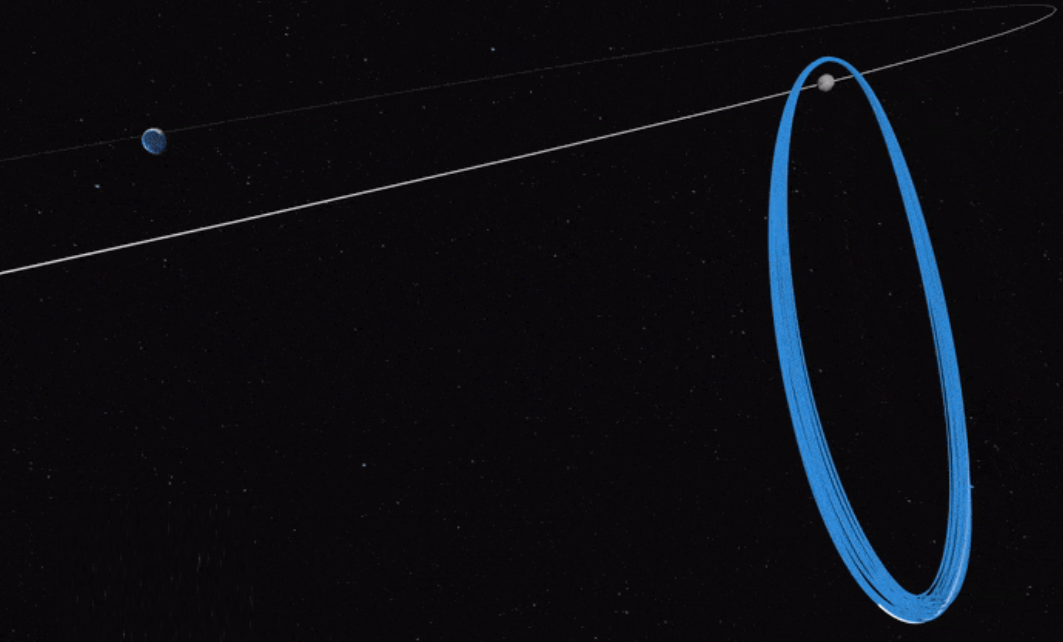
\includegraphics[width=1\linewidth]{1 Introducao/Imagens/Gateway lunar NRHO orbit.png}
    \caption{Demonstração da órbita do Lunar Gateway. Fonte: ESA.}
    \label{fig:orbitaGatewayNRHO}
\end{figure}

Para que toda a missão seja viável, é importante que os procedimentos de RVD/B entre os veículos espaciais e a estação sejam robustos e precisos, pois sem esse tipo de operação, a exploração futura não é possível.
No contexto do \emph{Lunar Gateway}, essas manobras permitirão a chegada de tripulações, cargas, módulos adicionais e outros equipamentos, além de que irá viabilizar o retorno dos veículos espaciais à Terra.